\documentclass[12pt]{article}
\usepackage{graphicx}
\usepackage{xcolor}
\usepackage{subfigure}
\usepackage[margin=1.0in]{geometry}
\usepackage{float}
\usepackage{amsmath}
\usepackage{mathtools}
\usepackage{wrapfig}
\usepackage{setspace}
\usepackage{multicol}
\renewcommand{\baselinestretch}{1.5}
\usepackage[utf8]{inputenc}
\usepackage{etoolbox}
\patchcmd{\thebibliography}{\section*{\refname}}{}{}{}
\author{Shivesh Pathak}
\title{Developing effective theories for single and bilayer graphene using density matrix downfolding}

\begin{document}
\maketitle
\begin{abstract}
A core problem of condensed matter physics is understanding how to develop low-energy effective models for realistic systems.
I believe that a density matrix downfolding (DMD) method \cite{Zheng2017} can be used to systematically build effective theories for such systems beginning with a high energy theory like the \textit{ab-initio} Hamiltonian.
I present as a preliminary result an effective Hamiltonian developed using DMD which can accurately reproduce the spectra and properties of the lowest lying excitations of the CuO molecule.
I propose using DMD to develop accurate model Hamiltonians for single and bilayer graphene.
My work will serve to mature the DMD method and take steps towards a model for the strongly correlated twisted bilayer graphene system.
\end{abstract}
Committee: Lucas Wagner, Smitha Vishveshwara, David Ceperley, Karin Dahmen

Pool: \textit{David Ceperley},\textit{ Brian DeMarco}, Smitha Vishveshwara, Andre Schleife, \textit{Karin Dahmen} 
\pagebreak

\section{Introduction}
Developing model Hamiltonians for realistic materials is a fundamental problem in modern condensed matter physics.
A model Hamiltonian is a simplified description of a real material which can accurately reproduce the low-lying eigenstates and energies of the material.
Accurate models give clear and direct indications of effective interactions within a material and underpin modern theoretical understanding of ideas like emergence and symmetry breaking.
On a practical level, calculations related to these low-lying eigenstates can be carried out on the much simpler model system and still yield accurate results reflective of reality.

Yet unresolved is a paradigm for building many-body model Hamiltonians which can describe realistic systems.
Band and Fermi liquid theory have been successful in accurately modeling systems where effective interactions are negligible at low energy scales.
These theories, however, fail in describing the low-energy excitations of strongly correlated systems like high Tc superconductors and twisted bilayer graphene (TBLG).
Many-body models like the Hubbard \cite{Hubbard1963}, Kanamori \cite{10.1143/PTP.30.275}, t-J \cite{Chao_1977} and Heisenberg models have been proposed to describe such strongly correlated systems, but their effectiveness in describing realistic materials is unclear.

Common approaches to building many-body theories for real materials involve density functional theory (DFT) \cite{PhysRev.140.A1133}.
One-body terms are obtained by projecting the solutions from the DFT band structure onto a single-particle basis \cite{PhysRevLett.87.047003}.
Two-body terms are developed by assuming a screened Coulomb interaction based on constrained DFT, RPA, or other methods \cite{PhysRevB.62.R16219, PhysRevB.70.195104, PhysRevB.88.075106}.
L\''{o}wdin methods and canonical transformations have also been used to develop effective theories \cite{doi:10.1063/1.4802766, PhysRevA.81.013402, doi:10.1063/1.2196410}.
While useful techniques, it is typically impossible to know whether models built from them accurately describe reality, as usually no clear estimate of model quality is provided.

I propose using a quantum Monte Carlo (QMC) density matrix downfolding (DMD) procedure to develop accurate many-body model Hamiltonians for single (SLG) and bi-layer (BLG) graphene systems.
Recent observations of a fractional quantum Hall effect \cite {Bolotin2009, Du2009} and plasmarons \cite{Bostwick999} in SLG as well as unconventional superconductivity \cite{Cao2018_2} and many-body insulating states \cite{Cao2018} in TBLG have spurred an interest in developing many-body models for graphene.
The DMD procedure provides a framework for developing such a many-body model using QMC calculations starting from the \textit{ab-initio} Hamiltonian 
\begin{equation}
\hat{H}_\text{ab} = -\frac{1}{2} \sum_{i} \nabla_i^2 -\frac{1}{2\mu}\sum_{I} \nabla_I^2 + \frac{1}{2}\sum_{ij} \frac{1}{|r_i - r_j|} + \frac{1}{2}\sum_{IJ} \frac{Z_I Z_J}{|R_I - R_J|} - \sum_{iJ}\frac{Z_J}{|r_i - R_J|},\ \mu = (M/m)
\label{Hab}
\end{equation}
where $i$ index electrons, $I$ ions, and energy in Hartree (Ha).
The procedure makes no assumptions about the form of microscopic electronic interactions in the system and reports a clear, statistical measure of model quality.
By developing many-body models for SLG and BLG, I hope to further the understanding of interactions in graphene like systems and the maturity of DMD for its application to other strongly correlated systems like TBLG.

\subsection{Density Matrix Downfolding (DMD)}
I begin by defining what a low-energy effective Hamiltonian and downfolding are.
Consider a Hamiltonian $\hat{H}$ defined on a Hilbert space $\mathcal{H}$.
A low-energy effective Hamiltonian is an operator $\hat{H}_\text{eff}$ which can accurately reproduce the spectra, up to a constant, and eigenstates of $\hat{H}$ on a subpsace $\mathcal{LE}$ of the Hilbert space $\mathcal{H}$.
Here $\mathcal{LE}$ is taken to be the span of the N lowest energy eigenstates of $\hat{H}$, and $\hat{H}_\text{eff}$ is a linear combination of Hermitian operators $\hat{d}_k$ with a constant energy shift $E_0$
\begin{equation}
\hat{H}_\text{eff} = \sum_{k} g_k \hat{d}_k  + E_0.
\label{eq:Heff}
\end{equation}
The objective of Hamiltonian downfolding is to construct such an $\hat{H}_\text{eff}$ given $\hat{H}, \mathcal{H}$.

The key insight of DMD is that the Hamiltonian downfolding problem can be mapped onto a linear regression problem.
It has been shown that the above definition of $\hat{H}_\text{eff}$ is equivalent to the following: a low-energy effective Hamiltonian is an operator on a subspace $\mathcal{LE}$ of $\mathcal{H}$ such that 
\begin{equation}
\begin{split}
\forall |\Psi\rangle \in \mathcal{LE},\ (E[\Psi] \equiv \langle \Psi|\hat{H} | \Psi \rangle)  = (E_\text{eff}[\Psi] \equiv \langle \Psi | \hat{H}_\text{eff} | \Psi \rangle) + \epsilon[\Psi]
\end{split}
\label{eq:DMD}
\end{equation}
where $\epsilon[\Psi]$ is the error in the effective theory.
Given the general linear form of $\hat{H}_\text{eff}$ seen in \eqref{eq:Heff}, 
the task of building an effective Hamiltonian then reduces to fitting a linear model that minimizes the error $\epsilon[\Psi]$ over $\mathcal{LE}$.
The independent variables (descriptors) in the fitting are expectation values of the operators $d_k[\Psi] \equiv \langle \Psi |\hat{d}_k|\Psi \rangle$ and the target variable is $E[\Psi]$.

This linear regression problem can be tackled in three steps, beginning with sampling states from $\mathcal{LE}$.
Ideally the linear regression would be conducted over the entire space $\mathcal{LE}$. 
In practice, the space is too large, and instead a representative sample set is drawn and used for fitting.
Generally, one cannot sample the true low-energy subspace, and low-energy wave functions are sampled from an approximate subspace $\mathcal{LE}^\prime$.
For each sampled state $|\Psi_s\rangle$, the quantities $E[\Psi_s], \{d_k[\Psi_s]\}$ are calculated to be used in the linear regression.
The sampling and calculation are typically done in QMC, but less accurate methods like DFT and Hartree-Fock can be used as well, resulting is less accurate models.

Next, a set of candidate descriptors which form the effective Hamiltonian are selected.
Descriptors will typically be selected if their values co-vary with the energy over the set of sampled states. 
Knowledge of the low-energy degrees of the freedom from experiment and physical intuition can help restrict the set of candidate descriptors further.
In principle there is no restriction on the form of the candidate operators other than Hermiticity, but second quantized operators are commonly used.
If so, an appropriate single particle basis to express the second quantized operators must be constructed.

Finally, the sampled data are used to fit the coefficients $\{g_k\}$ by linear regression.
A typical fitting workflow involves feature selection, model regression and model validation.
Feature selection methods for choosing appropriate descriptors can range from wrapper methods like orthogonal matching pursuit \cite{Cai2011} and principal component analysis \cite{pearson_karl_1901_1430636} to embedded methods like LASSO \cite{10.2307/2346178}, ridge \cite{doi:10.1137/S0895479897326432} and elastic net regularizations \cite{Zou05regularizationand}. 
Fitting the effective Hamiltonian usually involves an ordinary least squares linear regression, but the cost function can be altered.
Model validation can be carried out by calculating cross validated single parameter measures like R$^2$ scores which carry information about goodness of fit and overfitting.

Importantly, the fit effective Hamiltonian carries with it a quantitative measure of its validity.
The ability to quantify the accuracy of an effective Hamiltonian sets DMD apart from contemporary downfolding approaches which typically report only a final model.
Given the statistical nature of the fitting procedure, model quality assessment can be carried out and reported in exhaustive detail if one is interested.
Typically, however, single parameter measures like cross validated R$^2$ scores are used to quantify the accuracy of the effective Hamiltonian.

\subsection{Fixed-node diffusion Monte Carlo (FN-DMC)}
Diffusion Monte Carlo (DMC) is a quantum Monte Carlo method which projects out the ground state of a real-space Hamiltonian given some initial trial wave function.
Consider a trial wave function $|\Psi_T\rangle$ and the Hamiltonian $\hat{H}$ with ground state $|\Phi_0\rangle$. 
Applying the projector $e^{-\tau \hat{H}}$ as $\tau \rightarrow \infty$ to $|\Psi_T \rangle$
\begin{equation}
\lim_{\tau \rightarrow \infty} e^{-\tau \hat{H}} |\Psi_T\rangle 
\equiv \lim_{\tau \rightarrow \infty} |\Psi_\text{DMC}(\tau)\rangle \propto \langle \Phi_0|\Psi_T\rangle |\Phi_0\rangle,
\end{equation}
projects out the ground state as long as the trial wave function is not orthogonal to the ground state. 
DMC provides a stochastic implementation of this projector method and involves moving samples from the trial function $\Psi_T(R)$ using the Green function $G(R, R^\prime, \tau) = \langle R | e^{-\tau(\hat{H} - E_T)} | R^\prime \rangle$. 
Since $\hat{H} = \hat{T} + \hat{V}$, kinetic and potential energy terms, the Green function is approximated by a Trotter expansion 
$$G(R, R^\prime, \tau) = \langle R | e^{-\tau(\hat{H} - E_T)} | R^\prime \rangle \sim \Big[e^{-d\tau(\frac{V(R) + V(R^\prime)}{2} - E_T)} \langle R| e^{-d\tau\hat{T}}|R^\prime \rangle + O(d\tau^2) \Big]^N $$ 
where $d\tau = \tau/N$.
This expansion can be interpreted as an interative procedure where samples are moved N times with a small timestep $d\tau$ until convergence.
The constant $E_T$ is a trial energy used to control the normalization of $\Psi_\text{DMC}(\tau, R)$ and is updated at each move.

DMC, however, suffers from a fermion sign problem which is alleviated via a fixed-node approximation.
Under the fixed-node approximation the nodal surface of $\Psi_\text{DMC}(\tau, R)$ is forced to match that of the initial trial wave function for all $\tau$.
This approximation makes FN-DMC variational, and will only return the exact ground state of $\hat{H}$ if the nodal surfaces of $|\Psi_T\rangle$ and $|\Phi_0\rangle$ are identical.

One can take advantage of the variational nature of FN-DMC to sample the low-energy states necessary for DMD.
Consider a set of trial wave functions with varying nodal structures.
The final projected $\Psi_\text{DMC}$ for these different trial functions will be the lowest energy states in $\mathcal{H}$ for the given nodal structures.
If the initial trial wave functions are appropriately chosen, the final projected states will be low-energy states within $\mathcal{H}$.
The expectation values $E[\Psi_\text{DMC}], \{d_k[\Psi_\text{DMC}]\}$ necessary for the model regression are calculated using a mixed estimator.

\section{Preliminary Work}
\subsection{Non-orthogonal determinants in FN-DMC trial wave functions}
In order to become acquainted with our code QWalk \cite{Wagner2009} and QMC algorithms in general I worked on implementing and testing multi-Slater-Jastrow trial functions with optimized non-orthogonal determinants (MSJ+NO) in FN-DMC \cite{doi:10.1063/1.5052906}.
The MSJ+NO trial wave functions take the form
\begin{equation}
\Psi=e^{J(\vec{\alpha})} \sum_I e^{\hat{\Theta}(\vec{\theta_I})} C_I |D_I (\{ \phi\})\rangle
\end{equation}
where the determinants $|D_I\rangle$ are composed of single particle orbitals from a self-consistent field calculation, $e^J$ is a spin-independent Jastrow factor, $e^{\hat{\Theta}}$ is a spin-dependent orbital rotation matrix, and the wave function has variable parameters $\vec{\alpha}, \vec{\theta}, \vec{C}$ which can be optimized.

We assessed the efficiency and compactness of this new trial function by calculating the ground state energy and single particle densities of a C$_2$ molecule using FN-DMC and comparing to the results when using multi-Slater-Jastrow trial functions with optimized orthogonal determinant trial functions (MSJ+O). 
The workflow involved constructing the un-optimized trial wave functions, optimizing the parameters using an energy optimization method \cite{Toulouse2007}, and finally using the optimized trial functions in both variational Monte Carlo (VMC) and FN-DMC calculations. 
We found the average improvement in variational energy when using optimized orthogonal determinants is $\langle E_\text{MSJ} - E_\text{MSJ+O} \rangle = $ 0.32 eV with a standard deviation of 0.08 eV, with an additional improvement from the non-orthogonal determinants of 0.031 eV with a standard deviation of 0.021 eV.
The average improvement in the FN-DMC energy with the MSJ+O trial wave functions was 0.14 eV (standard deviation 0.03 eV) with an additional reduction of 0.032 eV (standard deviation 0.019 eV) when using the MSJ+NO trial wave function.

While the benefit using the MSJ+NO trial wave function seems small, we saw that the FN-DMC energy calculated using an MSJ+NO trial function with only 24 determinants was lower than the FN-DMC energy using an MSJ+O trial function with 55 determinants.
Further, the FN-DMC charge density calculated using MSJ+NO trial functions had stronger bonding character than when using MSJ+O trial functions, a reasonable result as introducing correlations into trial functions allows for electrons to avoid each other while still occupying the same bonding region. 
Our results indicated that using non-orthogonal determinants may lead to more compact multi-Slater-Jastrow trial wave functions for small molecules.

\subsection{Effective theory for CuO molecule using DMD}
As a first step towards developing accurate models for extended systems like solids using DMD, I constructed a many-body effective model for the CuO molecule by downfolding \eqref{Hab} under a Born-Oppenheimer approximation with fixed bond length $r_e$ = 1.725\r{A}.
In the following four sections I will detail the steps I took towards developing a model for the CuO molecule using DMD.
First, I discuss how low-energy states were sampled for the model regression.
This is followed by details of descriptor selection and single particle basis construction.
With the sampled data and candidate descriptors in hand, the feature selection and model fitting procedures are described.
I will conclude by comparing the solutions of the model Hamiltonian to experiment and previous theoretical calculations.

\paragraph{Sampling low-energy states}
For the CuO molecule, low-energy states were generated by using FN-DMC projected multi-Slater-Jastrow (MSJ) trial wave functions.
The trial wave functions took the form
\begin{equation}
|\Psi_T(\vec{p}) \rangle =  e^{J}\sum_{j} p_j|\text{D}_j\rangle,
\label{eq:sampling}
\end{equation}
where $e^J$ is a Jastrow factor, $|\text{D}_j\rangle$ are selected determinants which we discuss below, and $p_j$ are variable coefficients.
A single three-body Jastrow factor was used for all sampled states optimized on the lowest energy determinant $|\text{D}_0 \rangle$.
This significantly reduced the computational cost of the DMD method and is justified by noting that large variations in the Jastrow factor would move the state outside the low-energy space.

The determinants $|\text{D}_j \rangle$ were constructed from the orbitals of independent symmetry-targeted unrestricted Kohn Sham (UKS) calculations.
This choice was made to ensure that the three major low-energy variations seen in the molecule can be captured in our samples: occupancy, spin configuration and relaxation of the Cu 3d, 4s and O 2p orbitals.
All determinants with at most a single hole in the Cu 3d shell and no doubly occupied Cu 4s orbital were included in \eqref{eq:sampling} to reflect the low-energy excitations seen in experiment.
Only the lowest energy state with a Cu 4s$^2$ electronic configuration was included, corresponding to a double excitation 2 O ${2p_\pi} \rightarrow$ 2 Cu 4s with an energy $>7$ eV above the UKS ground state.
Inclusion of this high energy determinant is necessary so our model places similar Cu 4s$^2$ states high in energy.
The UKS calculations were done using PySCF \cite{Sun2018}, a B3LYP functional \cite{doi:10.1063/1.464304, PhysRevB.37.785}, Trail-Needs psuedopotential and VTZ Trail-Needs basis \cite{doi:10.1063/1.4811651}.

A shell sampling scheme was used to sample states from the selected approximate low-energy space.
We began by fixing the coefficient $p_0 = \sqrt{w}$ where $w \in \{1.0, 0.8, ..., 0.2\}$. 
For each choice of $w$ we sampled n = 5 states by randomly selecting the unassigned coefficients from independent, standard normal distributions such that $\sum_j p_j^2 = 1$. 
This procedure generated a uniform set of samples from spherical shells at decreasing radii in determinant space centered at $|\text{D}_0\rangle$.
We repeated this process centered at every determinant in \eqref{eq:sampling} resulting in a sample set of overlapping shells which fill $\mathcal{LE}^\prime$.

The final sampled MSJ states were projected using FN-DMC to generate our low-energy states.
The FN-DMC calculations were conducted with T-moves to ensure the variational principle holds while using pseudopotentials.
A timestep of $\tau = 0.01$ was used.
These calculations were done in QWalk \cite{Wagner2009}.

\paragraph{Selecting candidate descriptors}
We selected the following set of 1- and 2-body operators to construct our candidate descriptors based on our understanding of the low-energy excitations of the CuO molecule and our sampled states:
\begin{equation}
\begin{split}
\sum_{\sigma = \uparrow, \downarrow} \Bigg(\epsilon_{3d_\pi}\hat{n}_{3d_\pi,\sigma} + \epsilon_{3d_{z^2}}\hat{n}_{3d_{z^2},\sigma} +  \epsilon_{2p_z} \hat{n}_{2p_z,\sigma} + \epsilon_{2p_\pi}\hat{n}_{2p_\pi,\sigma} + \epsilon_{4s}\hat{n}_{4s,\sigma} +\\
t_\pi \hat{c}_{3d_\pi,\sigma}^\dagger \hat{c}_{2p_\pi,\sigma} + t_{dz} \hat{c}_{3d_{z^2},\sigma}^\dagger \hat{c}_{2p_z,\sigma}  + t_{sz}\hat{c}_{4s,\sigma}^\dagger \hat{c}_{2p_z,\sigma} + t_{sd}\hat{c}_{4s,\sigma}^\dagger \hat{c}_{3d_{z^2},\sigma} + \text{h.c.} + \Bigg)  \\
J_{sd}\sum_{i\in {\{\text{xy, xz, ...}}\}} \vec{S}_{4s} \cdot \vec{S}_{3d_i} + U_s \hat{n}_{4s,\uparrow}\hat{n}_{4s,\downarrow} + E_0.
\end{split}
\label{eq:models}
\end{equation}
The operator subscripts correspond to the intrinsic atomic orbital (IAO) basis elements constructed using the molecular orbitals in \eqref{eq:sampling}, and can be seen in \ref{fig:cuo_regr}a.

The parantheses of \eqref{eq:models} contain the full set of symmetry allowed 1-body operators within the Cu 3d, 4s and O 2p space.
These operators are required to describe the most basic single particle features seen in molecules like orbital occupations and hybridizations.
Two 2-body interaction terms are also considered: a Hund's coupling between Cu 4s and 3d orbitals and a Cu 4s Coulomb repulsion.
The prior term is motivated by the existence of a $\sim $ 0.5 eV Hund's coupling on the neutral copper atom.
Motivation for the latter comes from the FN-DMC energies of our sampled data.
We find that states with a Cu $3d^{10} 4s^{2}$ configuration lie at least 7 eV above our lowest energy sampled state, while the highest energy states with a $3d^{10} 4s^{1}$ configuration lie near 2 eV.

\begin{figure*}
\centering
%\hspace*{-0.25in}
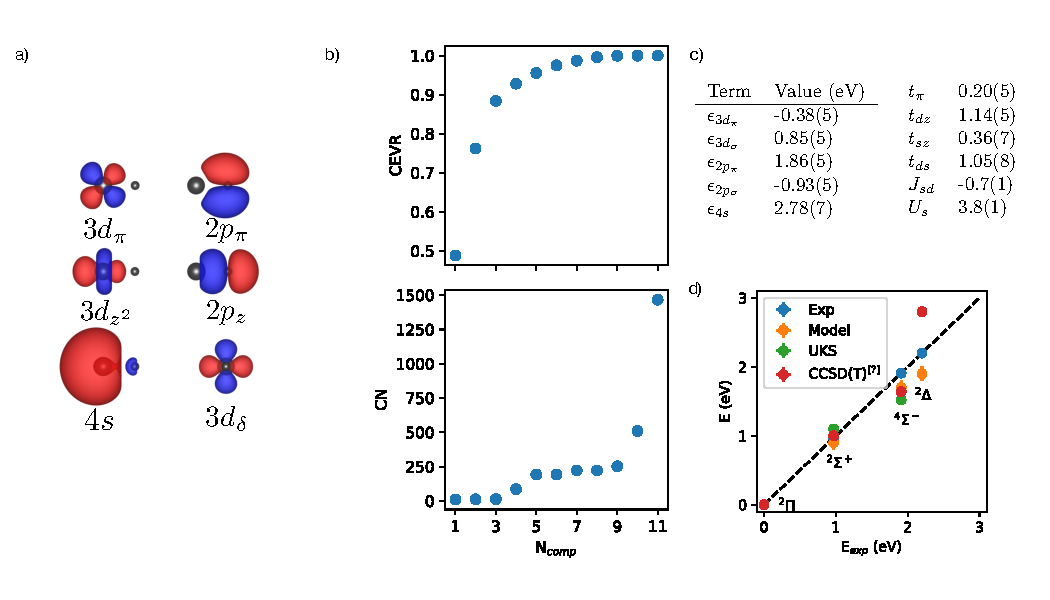
\includegraphics[width=1.0\linewidth]{./figs/cuo_regr_2.pdf}
\caption{Figures related to model regression for the CuO molecule: a) Intrinsic atomic orbitals used as a single particle basis for the model Hamiltonian, b) Results of PCA showing the CEVR and CN of a data set containing N$_{comp}$  highest ranked PCs, c) The final regressed parameters from the PCR, d) Comparison of four lowest lying eigenstates of CuO molecule between experiment and three computation methods.}
\label{fig:cuo_regr}
\end{figure*}

\paragraph{Fitting the model}
A direct attempt at fitting all eleven terms in \eqref{eq:models} leads to a high goodness of fit, R$^2$ = 0.99, but unexpectedly large coefficients for the fit model, like an enormous occupation energy gap of $\epsilon_{2p_\pi} - \epsilon_{3d_\delta} = $ 5.87 eV, which is 2 $-$ 3 eV in experiment and our sampled data.
This inflation of model parameters was found to be associated with multicollinearity among the candidate descriptors, quantified by a large condition number (CN) of 1470.

A principal component regression (PCR) was used to alleviate this multicollinearity and fit the effective theory \cite{10.2307/2348005}.
PCR can be broken into three parts: conducting a principal component analysis (PCA) and selecting candidate principal components to work with (PCs), fitting a linear model to these PCs, and then inverting the coefficients back to the original descriptors.
If the subset of PCs are chosen appropriately, the final regressed model will have a similar goodness of fit to one fit on the original data matrix but without the consequence of serious multicollinearity.

From the PCA, the nine highest ranked PCs were selected to use in the PCR.
In Figure \eqref{fig:cuo_regr}b we plot both the cumulative explained variance ratio (CEVR) and CN of a matrix composed of the $N_\text{comp}$ highest ranked PCs varying from one to eleven.
The CEVR indicates how much of the variation in the descriptor values a subset of PCs capture, and the CN quantifies the multicollinearity among these PCs.
The objective in selecting PCs is to the maximize the prior while simultaneously minimizing the latter, ensuring a high goodness of fit with little to no multicollinearity.
Nine principal components best satisfies the objective above with a CEVR 0.9995 and CN of 257.

The model fit to these nine PCs maintains an excellent goodness of fit without serious multicollinearity.
When trained on all the sampled data this model yields an $R^2$ = 0.98 with a CN of 257. 
An inverse PCA transformation was used to map the fit coefficients corresponding to the PC descriptors back into the original eleven coefficients of \eqref{eq:models}.
These coefficients can be seen in Figure \ref{fig:cuo_regr}c with single standard deviation bootstrap error estimates.

\paragraph{Solutions of the model}
The model is solved by exact diagonalization, and the solutions agree well with experimental spectra and state assignments.
Shown in Figure \ref{fig:cuo_regr}d is a comparison between the excitation energies calculated from our model and those seen in the latest anion photoelectron spectroscopy measurements \cite{Wu1997}.
The model energies for these eigenstates are denoted by orange circles and agree with experiment up to a maximum deviation of 0.2 eV.
The term symbols assigned in experiment also match the term symbols of the model eigenstates, which are constructed by looking at the multiplicity and electronic configuration of each model eigenstate. 

The model states also agree with recent theoretical calculations like UKS and CCSD(T).
The energies for the UKS and CCSD(T) \cite{Xian2000} states are shown in Figure \ref{fig:cuo_regr}d as green and red circles, respectively.
The UKS energies were calculated in this work in en route to constructing the determinants $|\text{D}_j\rangle$ used in our sampling scheme \eqref{eq:sampling}.
Our model energies agree with both theoretical techniques within errorbars for the first three states shown.
The energy of the highest energy $^2\Delta$ is severely over estimated using both UKS and CCSD(T), by nearly 1 eV.
This over estimation may arise from an inadequate relaxation of the $\sigma$ type orbitals which form a three orbital hybridization complex in this system.

\section{Proposed work}
My proposed plan involves building a sequence of model Hamiltonians for increasingly complicated graphene-like systems using QMC DMD, ending with BLG.
The systems I will be interested in are the benzene molecule, single layer graphene, AA stacked bilayer graphene and AB stacked bilayer graphene.
Conceptually, the benzene molecule is a kind of building block for SLG, and SLG is a building block for BLG, creating a sequence of systems from least to most complex.

The first system I will develop a model for is the benzene molecule, shown in Figure \ref{fig:proposed}a.
While relatively simple, this molecule shares many similarities with and forms the basic unit of SLG.
The delocalized $\pi$ orbitals in benzene carry over directly into SLG where they are the primary contributors to the well known Dirac bands.
Interaction effects seen in the benzene molecule are also reflected in SLG, such as on-site double occupation energies for the carbon atoms \cite{Zheng2017, Wagner2015}.
As such, developing a model for benzene will help me become familiar with model fitting for 2-D carbon based systems.

\begin{figure*}
\centering
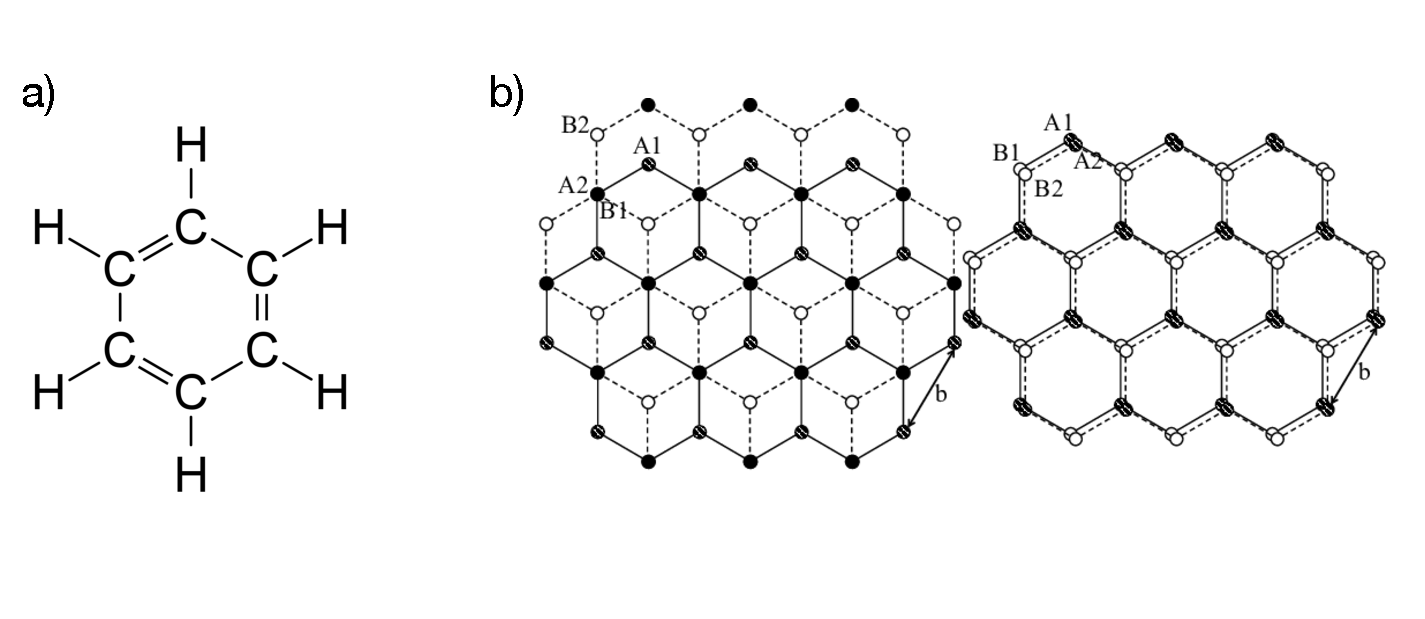
\includegraphics[width=1.0\linewidth]{./figs/proposed.pdf}
\caption{Schematic diagrams for the a) benzene molecule, b) AB and AA stacked BLG \textbf{ref}.}
%Voltage Tunable Plasmon Propagation in Dual Gated Bilayer Graphene
\label{fig:proposed}
\end{figure*}

The candidate descriptors I will use for DMD are motivated by a previous calculation on the benzene molecule \cite{Wagner2015}.
In that study, an extended Hubbard model built on the six $\pi$ orbitals was found to perform well in describing the low-lying excitations of the material.
The final model took the form 
\begin{equation}
H_\text{benz} = -\sum_{\langle i,j \rangle} t_{ij}c_i^\dagger c_j + U \sum_i n_{i\uparrow}n_{i\downarrow}  + \sum_{\langle i,j \rangle}V_{ij} n_i n_j + \sum_{\langle \langle i,j \rangle\rangle}V_{ij} n_i n_j
\label{Hbenz}
\end{equation}
where the brackets denote nearest neighbor and next-nearest neighbor summations.
I will consider at least all the descriptors above and also longer range hopping terms.

The second system I will be interested in working on is SLG.
Single layer graphene is composed of a triangular Bravais lattice with two carbon atoms per unit cell.
In terms of a non-interacting picture, the $\sigma$ orbitals composed of C $2s, 2p_x,$ and $2p_y$ lie below the Fermi level.
The bands which cross the Fermi level, and compose the distinct Dirac cones seen in SLG, are primary $\pi$ bonded molecular orbitals composed of C $2p_z$ orbitals.
Further, reduced screening in SLG leads to long range Coulomb interactions in the system \cite{Elias2012, Yu2013}.

In particular, I will work to extend a previous on-site Hubbard model developed for SLG \cite{Zheng2017, Wagner2015} by including long range density-density interactions .
The candidate model will be of the form:
\begin{equation}
H_\text{SLG} = -\sum_{i,j} t_{ij}c_i^\dagger c_j + U \sum_i n_{i\uparrow}n_{i\downarrow}  + \sum_{i,j} V_{ij} n_i n_j
\label{Hslg}
\end{equation}
where the indices correspond to the $\pi$ orbitals on the copper atoms.
I will consider both long range hopping and density-density interaction terms extending across the computational unit cell with the final goal of developing position dependent parameter values $t(r), V(r)$.

The last systems I will develop models for are AA and AB stacked BLG, shown in Figure \ref{fig:proposed}b.
AA stacked BLG is simply two sheets of graphene placed on top of one another where each atom is aligned with the atom beneath it.
In AB stacked BLG, a carbon atom from the lower layer is present in the center of each carbon hexagon of the upper layer, and vice versa.
As such, one can think of AB BLG as a shifted version of AA BLG, where the shift is half the size of a single carbonic hexagon.

I anticipate that the candidate descriptors should include interlayer couplings as well as the terms seen in SLG.
As such, the candidate model for BLG would be
\begin{equation}
H_\text{BLG} = H_\text{SLG}^{(1)} + H_\text{SLG}^{(2)} - \sum_{i_1, i_2} t_{i_1, i_2}^\prime c_{i_1}^\dagger c_{i_2} + h.c.
\label{Hblg}
\end{equation}
There are two terms for the single layers from \eqref{Hslg} plus an interlayer hopping given by the term $t_{i_1, i_2}^\prime.$
I suspect that the hopping values will be very different between the AA and AB models as the distance between interlayer neighbors differs greatly between the two stackings.
This difference in value will provide the first steps into developing model parameters for BLG which depend on the relative orientation of the sheets.

A new constrained variational Monte Carlo (cVMC) method will be used to sample the low-energy wave functions necessary for DMD.
The cVMC method works by minimizing the following cost function for a parameterized wave function $|\Psi(\vec{p})\rangle$:
\begin{equation}
\vec{p}^* = \text{argmin} \ \langle \Psi(\vec{p}) | \hat{H}_\text{ab} | \Psi(\vec{p}) \rangle - \vec{\lambda} \cdot \langle \Psi(\vec{p}) | (\vec{d} - \vec{d}_0)^2 | \Psi(\vec{p}) \rangle 
\end{equation}
with respect to the parameters $\vec{p}$.
The quantity $\vec{d}$ is short hand for a list of candidate descriptors to sample variations in, $\vec{d}_0$ is the target values of those candidate descriptors, and $\vec{\lambda}$ controls the importance of finding a state with low-energy versus one with descriptor values near $\vec{d}_0$.
Essentially this method allows us, for a given parameterization of $|\Psi(\vec{p})\rangle$, to generate low-energy wave functions which sit near a target point $\vec{d}_0$ in candidate descriptor space.

I will use a multi-Slater-Jastrow (MSJ) parameterization in the cVMC sampling for each system.
The multi-Slater expansion will consist of determinants of single particle orbitals calculated using DFT.
The determinants will include the DFT ground state as well as molecular orbital excitations among the $\pi$ and $\pi^*$ orbitals which form the active space.
A three body Jastrow factor will be applied to ensure that correlations are included in the wave function and that the wave function is low in energy.
The total set of parameters $\vec{p}$ will include both Jastrow and determinental coefficients.

Apart from their individual value, the four models can be used to investigate the transferrability of model parameters between these different carbon-based systems.
The first question would be whether the parameter values between a finite size system, like benzene, match those seen in the bulk SLG system.
The second would be whether the intralayer parameter values change in each sheet of SLG when they are brought together in the AA and AB configuration.
The latter question hints at a broader question, whether the SLG intralayer parameters are transferrable to TBLG, especially near the magic twist angles where interlayer coupling becomes very large \cite{Bistritzer2011}.

Further, my calculations will help mature methods like cVMC for further usage on strongly correlated systems.
A few questions of interest include how one should select values like $\vec{\lambda}$ and $\vec{d}_0$, and whether final models fit with cVMC are consistent with those fit previously using a different sampling technique.
The prior question will be naturally investigated while using cVMC in building models for the systems above.
The latter can be directly probed by comparing my fit models for benzene and on-site SLG to those which were developed previously using DMD.

Lastly, my calculations will lay the groundwork for model development for the strongly correlated TBLG system using DMD.
The final goal for TBLG would be an interacting continuum model on the Moire superlattice length scale.
From a DMD perspective, this can accomplished by first downfolding the \textit{ab-initio} Hamiltonian with a given twist to an atomic length scale model, and then downfolding a second time to the Moire length scale.
Developing the atomic length scale models requires a strong understanding of intra- and inter-layer interactions in this material.
The prior will be thoroughly investigated by my model fitting on SLG, and I will begin to answer the latter with the BLG calculations.

\paragraph{Proposed timeline} I believe that developing effective theories for the benzene molecule, SLG, AA and AB stacked BLG should take 2 years. 
The model fitting for benzene should take no more than four months.
The goal is to reproduce prior DMD calculations for the same material while benchmarking and familiarizing myself with the new cVMC sampling technique that I will use extensively in my project.
The SLG model fitting should take another eight months.
This is an extension of a previous work, and the first three months will be dedicate to reproducing the results from that work, namely a single band on-site Hubbard model.
Inclusion of long range Coulomb interactions into the effective theory should take another three months.
The last two months will be geared towards finite size extrapolation in order to ensure the final model is applicable to bulk systems.
The last year of the project will be geared towards the AA and AB stacked BLG, with each project taking about six months to complete.
For each stacking, I expect four months will be necessary to build an effective theory, and the final two months will be dedicated to finite size extrapolation.

\begin{multicols}{2}
\begin{spacing}{0.5}
{\fontsize{10}{5}\selectfont
\bibliography{biblio}
\bibliographystyle{unsrt}
}
\end{spacing}
\end{multicols}
\end{document}